\chapter{Results}\label{chap:Results}
Regarding the Scholar Plot (SP), we ran a user survey and a focus group. The former had primarily a validating purpose. The latter aimed to elicit detailed feedback and ideas for further improving Scholar Plot. 

% =============================================================================
\section{Usability Feedback}
% =============================================================================

A total of 15 participants from various disciplines including Natural Sciences, Social Sciences, Life Sciences and Computer Science evaluated Scholar Plot. We asked each participant to review the interface and then complete an online survey. Special care was taken to ensure that the participants had correct understanding about the visualization component before they began rating. The participants answered the questions on a Likert scale from 1 to 5 with 1 being strongly disagree and 5 being strongly agree.

Figure \ref{fig:UserStudy} illustrates the mean evaluation for each visualization component. Accuracy, Usability and understandability of Scholar Plot scored the highest $(\mu = 4.2)$ as it is very intuitive and can be used with minimal assistance. Many participants gave us feedback that they mostly liked the visual scheme of Scholar Plot. Another observation is that the participants agree to use Scholar Plot to evaluate themselves $(\mu = 4.1)$. They suggested that Scholar Plot can be improved by adding more funding agencies. Overall, this evaluation indicated that Scholar Plot is a user-friendly tool that complements the CV which can be used to review a scholar's accomplishments. The survey has been approved by the University of Houston Institutional Review Board (IRB). The survey form is available at \url{https://goo.gl/v7zHp5}
 
 \begin{figure}
  \centering
  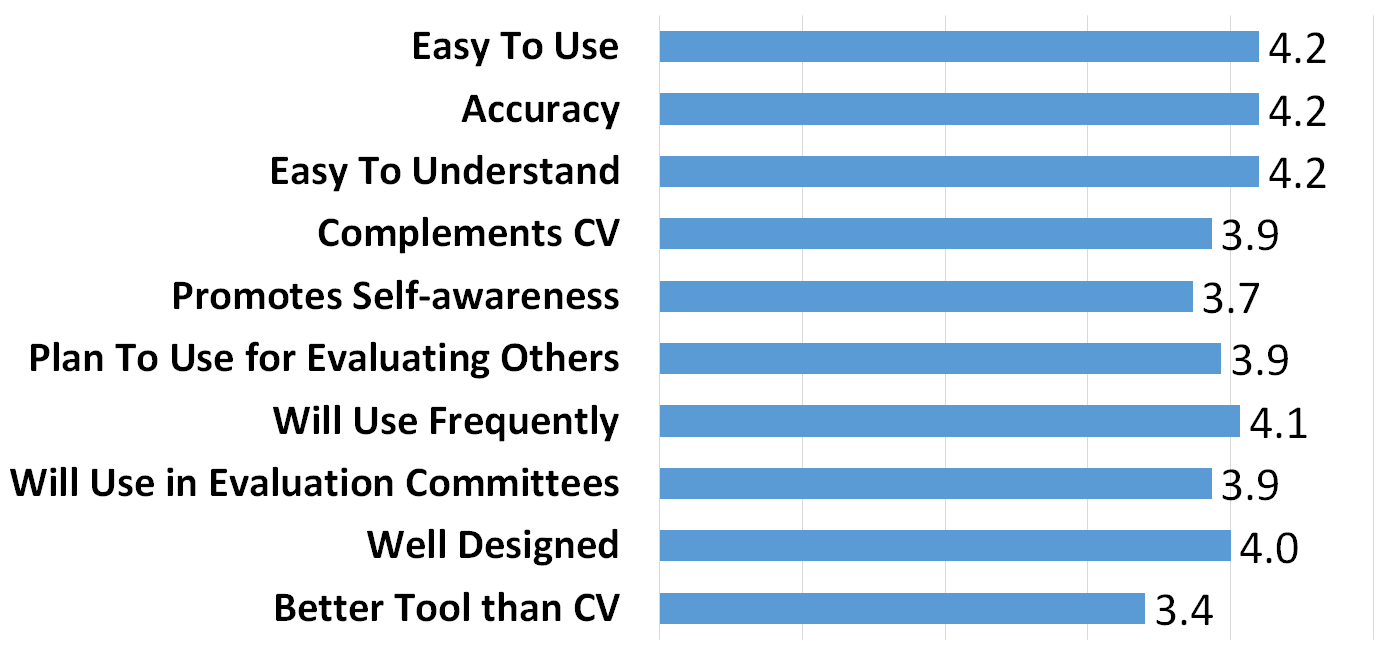
\includegraphics[width=\columnwidth]{figures/fig_survey_chart}
  \caption{Mean evaluation of Scholar Plot. A total of $n=15$ participants evaluated the survey.}
  \label{fig:UserStudy} 
\end{figure}

 \begin{figure}
  \centering
  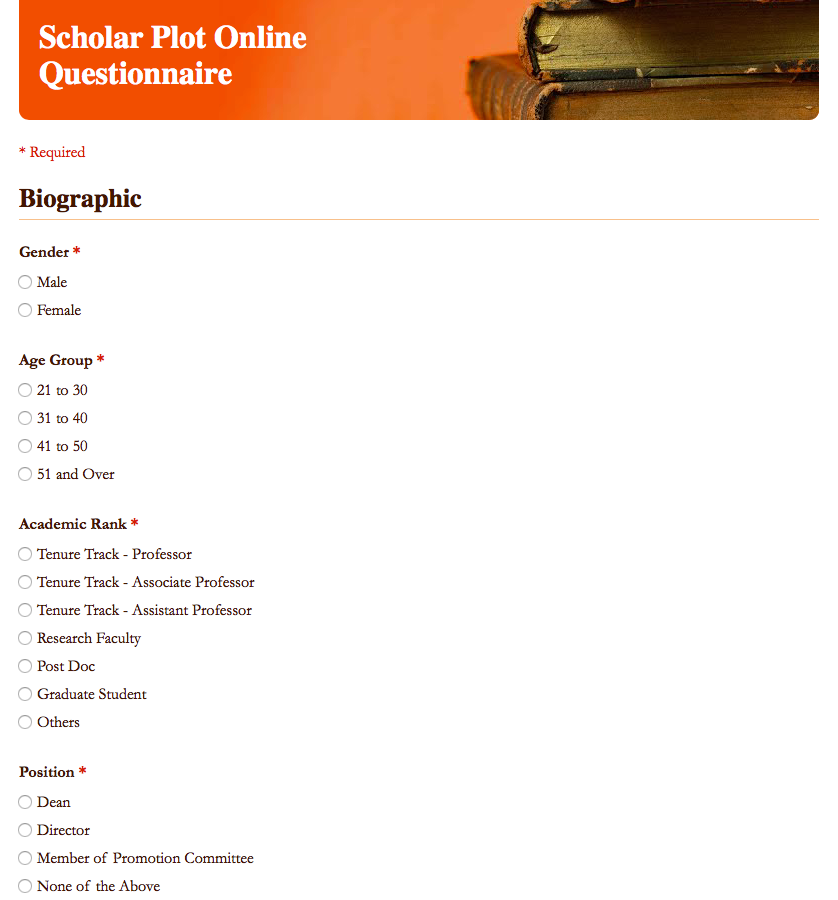
\includegraphics[width=\columnwidth]{figures/fig_survey_form}
  \caption{A part of sections of online survey form for User Study}
  \label{fig:SurveyForm} 
\end{figure}

% =============================================================================
\subsection{User Feedback - Focus Group}
% =============================================================================
We ran a focus group with 10  Principal Investigators and their post docs at Northwestern University. The participant set included biologists, physicists, computer scientists, and social scientists.  The focus group's suggestions are synopsized as follows:
\begin{description}
\item [Interface team science information.] Participants wanted to see the number and intensity of collaborations for the depicted scholar.
\item [Summarize highly cited papers.] Participants wanted to see explicitly in a side panel the scholar's most popular papers.
\item [Interface journal profile.] Participants wanted to see the specific journals where the scholar publishes most often and their impact factors.
\end{description}

 \begin{figure}[h]
  \centering
  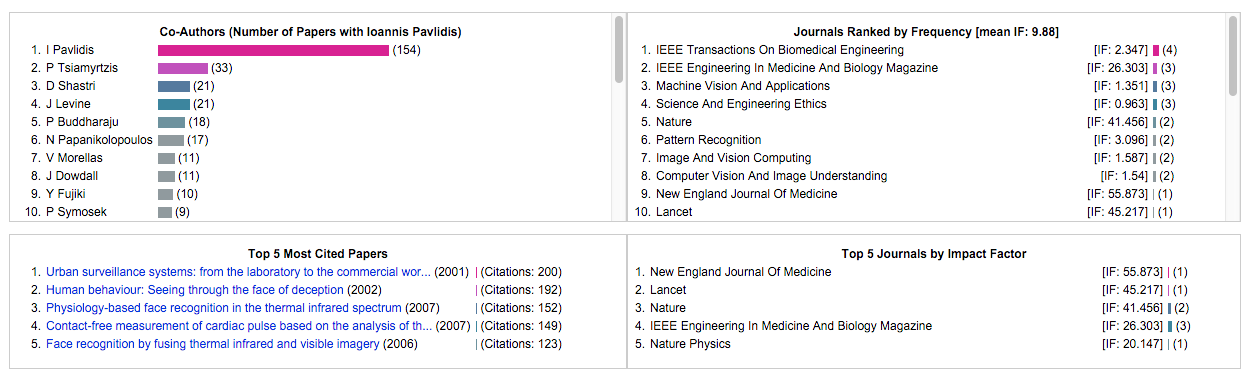
\includegraphics[width=\columnwidth]{figures/fig-panels}
  \caption{Four ancillary panels - Team, Impact, Prestige}
  \label{fig:panels} 
\end{figure}

The participants believed that accessorizing the central publication graph with this additional information would support deeper instant insights without compromising the elegance of SP's compact visual representation. Specifically, this additional interface would reveal the collaborative nature of the scholar's work, give hints if s/he is regular in specific disciplinary journals or if s/he publishes in a variety of journals (interdisciplinarity), and give the rank of these journals. All this information can also be gleaned by rolling the mouse over the publication graph, reading the tooltips; summarizing it in panels under the graph, however, renders such manual investigation unnecessary.